\chapter{Lasery półprzewodnikowe}
\section{Teoria}
\subsection{Teoria pasmowa}
Działanie laserów półprzewodnikowych opiera się na prawach, które opisuje teoria pasmowa.
Podstawowe przewidywanie teorii pasmowej mówi, że ciało stałe składa się z szeregu pasm rozdzielonych od siebie
przerwami energetycznymi o skończonych szerokościach wyrażanych w eV. Najważniejszą przerwą, która ma wpływ na właściwości elektryczne ciała jest
przerwa pomiędzy pasmem walencyjnym i pasmem przewodnictwa tzw. przerwa energii wzbronione $E_g$. Ze względu na szerokość przerwy
wyróżniamy ~\cite{laser_book}:
\begin{itemize}
\item izolatory: $E_g > 3$\,eV
\item półprzewodniki: $E_g =$ 0.1\,eV--2.5\,eV
\item przewodniki: $E_g<$0.1\,eV
\end{itemize}
Wartość przerwy energetycznej maleje z temperaturą według zależności ~\cite{laser_book}:
\begin{equation}
E_g(T) = E_{g0} - \frac{\alpha T^2}{\beta + T}
\end{equation}
gdzie: $E_{g0}$ --- wartooś przerwy energetycznej w temperaturze $T=0$\,K, \\ $\alpha = 4.5 \cdot 10^{-4}$\,eV/K.
Wartość parametru $\beta$ jest dodatnia i zależny od rodzaju półprzewodnika, więc im wyższa temperatura tym wartość przerwy mniejsza.
\subsection{Lasery półprzewodnikowe}
Lasery półprzewodnikowe są ważną oraz dynamicznie rozwijająca się gałęzią optoelektroniki. Cały czas są one udoskonalane, dzięki czemu obejmują corasz szerszy zakres częstości widma oraz potrafią generować promieniowanie o dużych mocach.
Aby móc udoskonalać potrzebne są prace zarówno teoretyczne, jak i doświadczalne. Praca ta skupia się na części doświadczalnej.
Lasery półprzewodnikowe znajduje zastosowanie w telekomunikacji, zapisie informacji.
Zalety laserów półprzewodnikowych:
\begin{itemize}
\item małe wymiary
\item łatwość modulacji emitowanego promieniowania
\item niezawodność pracy
\item proste zasilanie
\end{itemize}
 \newpage
Lasery półprzewodnikowe inaczej nazywane kwantowe generatory optyczne są laserami złączowymi. Lasery te są źródłem
monochromatycznego oraz skolimowanego promieniowania spójnego. W tego typu laserach ośrodkiem aktywnym jest półprzewodnik.
Obszar czynny zazwyczaj ograniczony jest do wąskiego paska oraz położony jest w płaszczyźnie złącza p-n.
Pompowanie uzyskiwane jest przez wstrzykiwanie mniejszościowych nośników ładunku do obszaru p-n, które spolaryzowane jest w kierunku przewodzenia.
Rezonator jest zazwyczaj w kształcie prostopadłościanu o wymiarach ułamków milimetra, zazwyczaj wykonany także w materiale półprzewodnikowym\cite{publikcja_nakwaski}.
Sprężenie optyczne uzyskiwane jest przez zastosowanie pary zwierciadeł prostopadłych do płaszczyzny obszary czynnego lub
za pomocą pofałdowanej specjalnie powierzchni, która jest równoległa do tego obszaru (DFB - Distributed Feed Back).
Aby zaszła akcja laserowa, prąd zasilający musi przekroczyć pewną wartość progową zwaną prądem progowym $I_{\mathrm{th}}$, który w dalszej części jest
opisywany bardziej szczegółowo.
Podstawowym zjawiskiem fizycznym na których swe działanie opierają lasery półprzewodnikowe jest przejście promieniste, czyli proces rekombinacji elektronu i dziury w wyniku którego następuje emisja promieniowania. Gdy prąd osiągnie wystarczająco
dużą wartość dochodzi do inwersji obsadzeń, czyli stanu w którym liczba cząstek o wyższej energii jest większa niż cząstek o energiach niższych.
 Zajście inwersji obsadzeń pozwala wywołać akcję laserową. Emitowana wiązka światła charakteryzuje się niewielką rozbieżnością kątową (kilku stopni). Wśród laserów półprzewodnikowych
wyróżniamy: lasery VCSEL oraz lasery o emisji krawędziowej.

W półprzewodniku występuje także wiele mechanizmów rekombinacji niepromienistej~\cite{praca_dok}, w których energia wzbudzenia zamieniana
jest na drgania sieci krystalicznej, jednym z takich procesów jest rekombinacja Auger. W procesie rekombinacji Auger energia, która
powstała na skutek rekombinacji elektronu z dziurą jest przekazywana trzeciej cząstce: elektronowi lub dziurze, która wzbudzana jest
na wyższy poziom w obrębie swojego pasma. Wzbudzona w ten sposób cząstka na skutek relaksacji emituje fonony, wraz ze wzrostem temperatury
emisja fononów jest większa. Proces ten ma duże znaczenie dla sprawności laserów półprzewodnikowych oraz dla wartości prądu progowego.

\subsection{Laser VCSEL}
Lasery VCSEL (ang. \textit{Vertical Cavity Surface Emitting Laser}) jest to laser z emisją powierzchniową o pionowej wnęce rezonansowej.
W laserach VCSEL promieniowanie rozchodzi się w kierunku prostopadłym do krawędzi obszaru czynnego oraz wzmacniane jest jedynie
wewnątrz tego obszaru\cite{publikcja_nakwaski}. Zaletami laserów VCSEL~\cite{publikcja_nakwaski} są
\begin{itemize}
\item mała rozbieżość wiążki promieniowania,
\item naturalna praca na pojedynczym modzie podłużnym
\end{itemize}
Wadami laserów VSCEL~\cite{publikcja_nakwaski} są
\begin{itemize}
\item bardzo niskia moc promieniowania wyjściowego
\item Stosunkowa wysoka wartość oporności elektrycznej i cieplnej
\end{itemize}
\subsection{Laser o emisji krawędziowej}
Laser krawędziowy są to laser z wnęka w płaszczyźnie warstwy aktywnej. W tego typach laserów promieniowanie wędruje w rezonatorze między
jego zwierciadłami, jednocześnie cały czas znajdując się wewnątrz ośrodka czynnego. Zaletami laserów krawędziowych są:
\begin{itemize}
\item Stosunkowa wysoko moc wiązki wyjściowej\cite{publikcja_nakwaski},
\item Stosunkowa wysoka sprawność.
\end{itemize}
Wadami laserów krawędziowych są~\cite{publikcja_nakwaski}:
\begin{itemize}
\item wzbudzanie się wielu modów podłużnych,
\item rozbieżna wiązka promieniowania, która wykazuje astygmatyzm.
\end{itemize}
\subsection{Prąd progowy}
Charakterystyka wyjściowa lasera przedstawia zależność napięcia na laserze oraz mocy wyjściowej w funkcji aplikowanego prądu.
Ważnym parametrem laserów półprzewodnikowych jest prąd progowy (z ang. \textit{threshold
current}) który określa wartość prądu, przy którym zaczyna zachodzić akcja laserowa, czyli
rośnie gwałtownie natężenie promieniowania i maleje szerokość linii emisyjnej. W celu wyznaczenia prądu progowego należy
sporządzić wykres zależności mocy wyjściowej lasera od prądu zasilającego. Następnie dla prądu gdzie zaczyna się akcja
laserowa dla odcinka liniowego należy metodą najmniejszych kwadratów przy użyciu wielomianu pierwszego stopnia(\ref{eq:fit_i_th})
znaleźć parametry prostej o parametrach $a$ i $b$.
Dla wyznaczonej krzywej należy znaleźć miejsce zerowe, które będzie wyznaczonym prądem progowym $I_{\mathrm{th}}$(\ref{eg:i_th}).
\begin{equation}
\label{eq:fit_i_th}
P_{wy} = a \cdot I + b
\end{equation}
\begin{equation}
\label{eg:i_th}
I_{\mathrm{th}} = -\frac{b}{a}
\end{equation}
\begin{equation}
\Delta I_{\mathrm{th}} = \left\lvert \frac{\partial I_{th}}{\partial a} \right\rvert \cdot \Delta a + \left\lvert \frac{\partial I_{th}}{\partial b} \right\rvert \cdot \Delta b
\end{equation}
\begin{equation}
\Delta I_{\mathrm{th}} = \left\lvert -\frac{b}{a^2} \right\rvert \cdot \Delta a + \left\lvert -\frac{1}{a} \right\rvert \cdot \Delta b
\end{equation}
Dla laserów krawędziowych prąd progowy rośnie wraz z temperaturą, co może być scharakteryzowane za pomocą parametru
$T_{0}$ wyrażonego w kelwinach tzw. temperatury charakterystycznej~\cite{opto_book}.
Dla laserów krawędziowych zależności prądu progowego $I_{th}$ od temperatury $T$ wyrażamy w postaci równania:
\begin{equation}
\label{eq:i_th}
I_{\mathrm{th}} = I_0 \exp \left( \frac{T}{T_0} \right)
\end{equation}
Przez zlogarytmowanie wartości prądu oraz podstawienie otrzymujemy:
\begin{equation}
\ln(I_{\mathrm{th}}) =    \frac{T}{T_0}  + \ln(I_0)
\end{equation}
Wartości parametrów $I_0$ oraz $T_0$ możemy wyznaczyć na podstawie charakterystyk
emisyjnych lasera w różnych temperaturach $T$. \\
Mając wartości prądu progowego w danej temperaturze  można do nich dopasować funkcje liniową w postaci:
\begin{equation}
y = a \cdot T + b
\end{equation}
Gdzie:
\begin{equation}
y = \ln(I_{\mathrm{th}})
\end{equation}
\begin{equation}
a = \frac{1}{T_0}
\end{equation}
\begin{equation}
b = \ln(I_0)
\end{equation}
Na tej podstawie możemy znaleźć poszukiwane parametry $I_0$ oraz $T_0$:
\begin{equation}
I_0 = \mathrm{e}^b
\end{equation}
\begin{equation}
T_0 = \frac{1}{a}
\end{equation}
Korzystając z metody różniczki zupełnej można obliczyć wartości błędów wyznaczonych wartości:
\begin{equation}
\Delta I_0 = \left\lvert \frac{\partial I_{0}}{\partial b} \right\rvert \cdot \Delta b = | \mathrm{e}^b | \cdot \Delta b
\end{equation}
\begin{equation}
\Delta T_0 = \left\lvert \frac{\partial T_{0}}{\partial a} \right\rvert \cdot \Delta a = \left\lvert -\frac{1}{a^2} \right\rvert \cdot \Delta a
\end{equation}
Dla laserów VCSEL nie można zastować powyszej zależności (\ref{eq:fit_i_th}).
\subsection{Sprawność}
Innym ważnym parametrem, którym możemy scharakteryzować lasery półprzewodnikowe jest ich sprawność. Można wyróżnić następujące rodzaje sprawności:
\begin{itemize}
\item Sprawność różniczkowa (ang. \textit{slope efficiency}) --- jest zdefiniowana jako nachylenie krzywej uzyskanej przez wykreślenie zależności
mocy wyjściowej $P_{wy}$ z lasera versus energii dostarczonej do lasera w postaci natężenie prądu $I$ lub mocy dostarczonej $P_{we}$.
Moc dostarczoną definujemy jako:
\begin{equation}
P_{we} = U \cdot I
\end{equation}
gdzie: $U$ --- napięcie na laserze. \\
Sprawność różniczkowa jest pochodną mocy wyjściowej po prądzie $\frac{dP_{wy}}{dI}$ lub pochodną mocy wyjściowej po mocy wejściowej $\frac{dP_{wy}}{dP_{we}}$
\item Sprawność całkowita (ang. \textit{wall-plug-efficiency}) --- jest zdefiniowana jako stosunek mocy wyjściowej do całkowitej mocy wejściowej lasera.
\end{itemize}
\newpage
\subsection{Funkcja Fermiego}
Na sprawność laserów półprzewodnikowych duży wpływ ma funkcja rozkładu Fermiego-Diraca przedstawiony na rysunku~\ref{fig:teoria_rys_3}. Funkcja Fermiego-Diraca opisuje prawdopodobieństwo obsadzenia przez elektron poziomu
energetycznego $E$ przy temperaturze $T$
\begin{equation}
\label{eq:fermi}
f(E) = \frac{1}{e^{(E-E_F)/kT} + 1}
\end{equation}
gdzie: $E_f$ --- energia Fermiego. \\
Energia Fermiego --- jest to energia najwyżej obrządzanego pasma w temperaturze 0\,K. Reprezentuje średnią pracę jakom należy wykonać
, aby usunąć elektrony z materiału. W temperaturze 0\,K poziom energii Fermiego dla samoistnego półprzewodnika znajduję się pośrodku pasmo walencyjnego i
pasma przewodnictwa. Wraz ze wzrostem temperatury przesuwa się w kierunku pasmo przewodnictwa, gdy jest przewodnictwo elektronowe lub
w kierunku pasma walencyjnego dla przewodnictwa dziurowego.
Zgodnie z równaniem ~\ref{eq:fermi} wraz ze wzrostem temperatury rośnie prawdopodobieństwo obsadzenia wyższych stanów energetycznych przez elektron. Ma to
negatywny wpływ na sprawność różniczkową lasera półprzewodnikowego. Ponieważ gdy temperatura rośnie, to więcej stanów o
wyższych energiach jest obsadzane, konsekwencją tego faktu jest mniejsza energia emitowanego promieniowania powstającego na
skutek rekombinacji promienistej.
\begin{figure}[H]
\center
  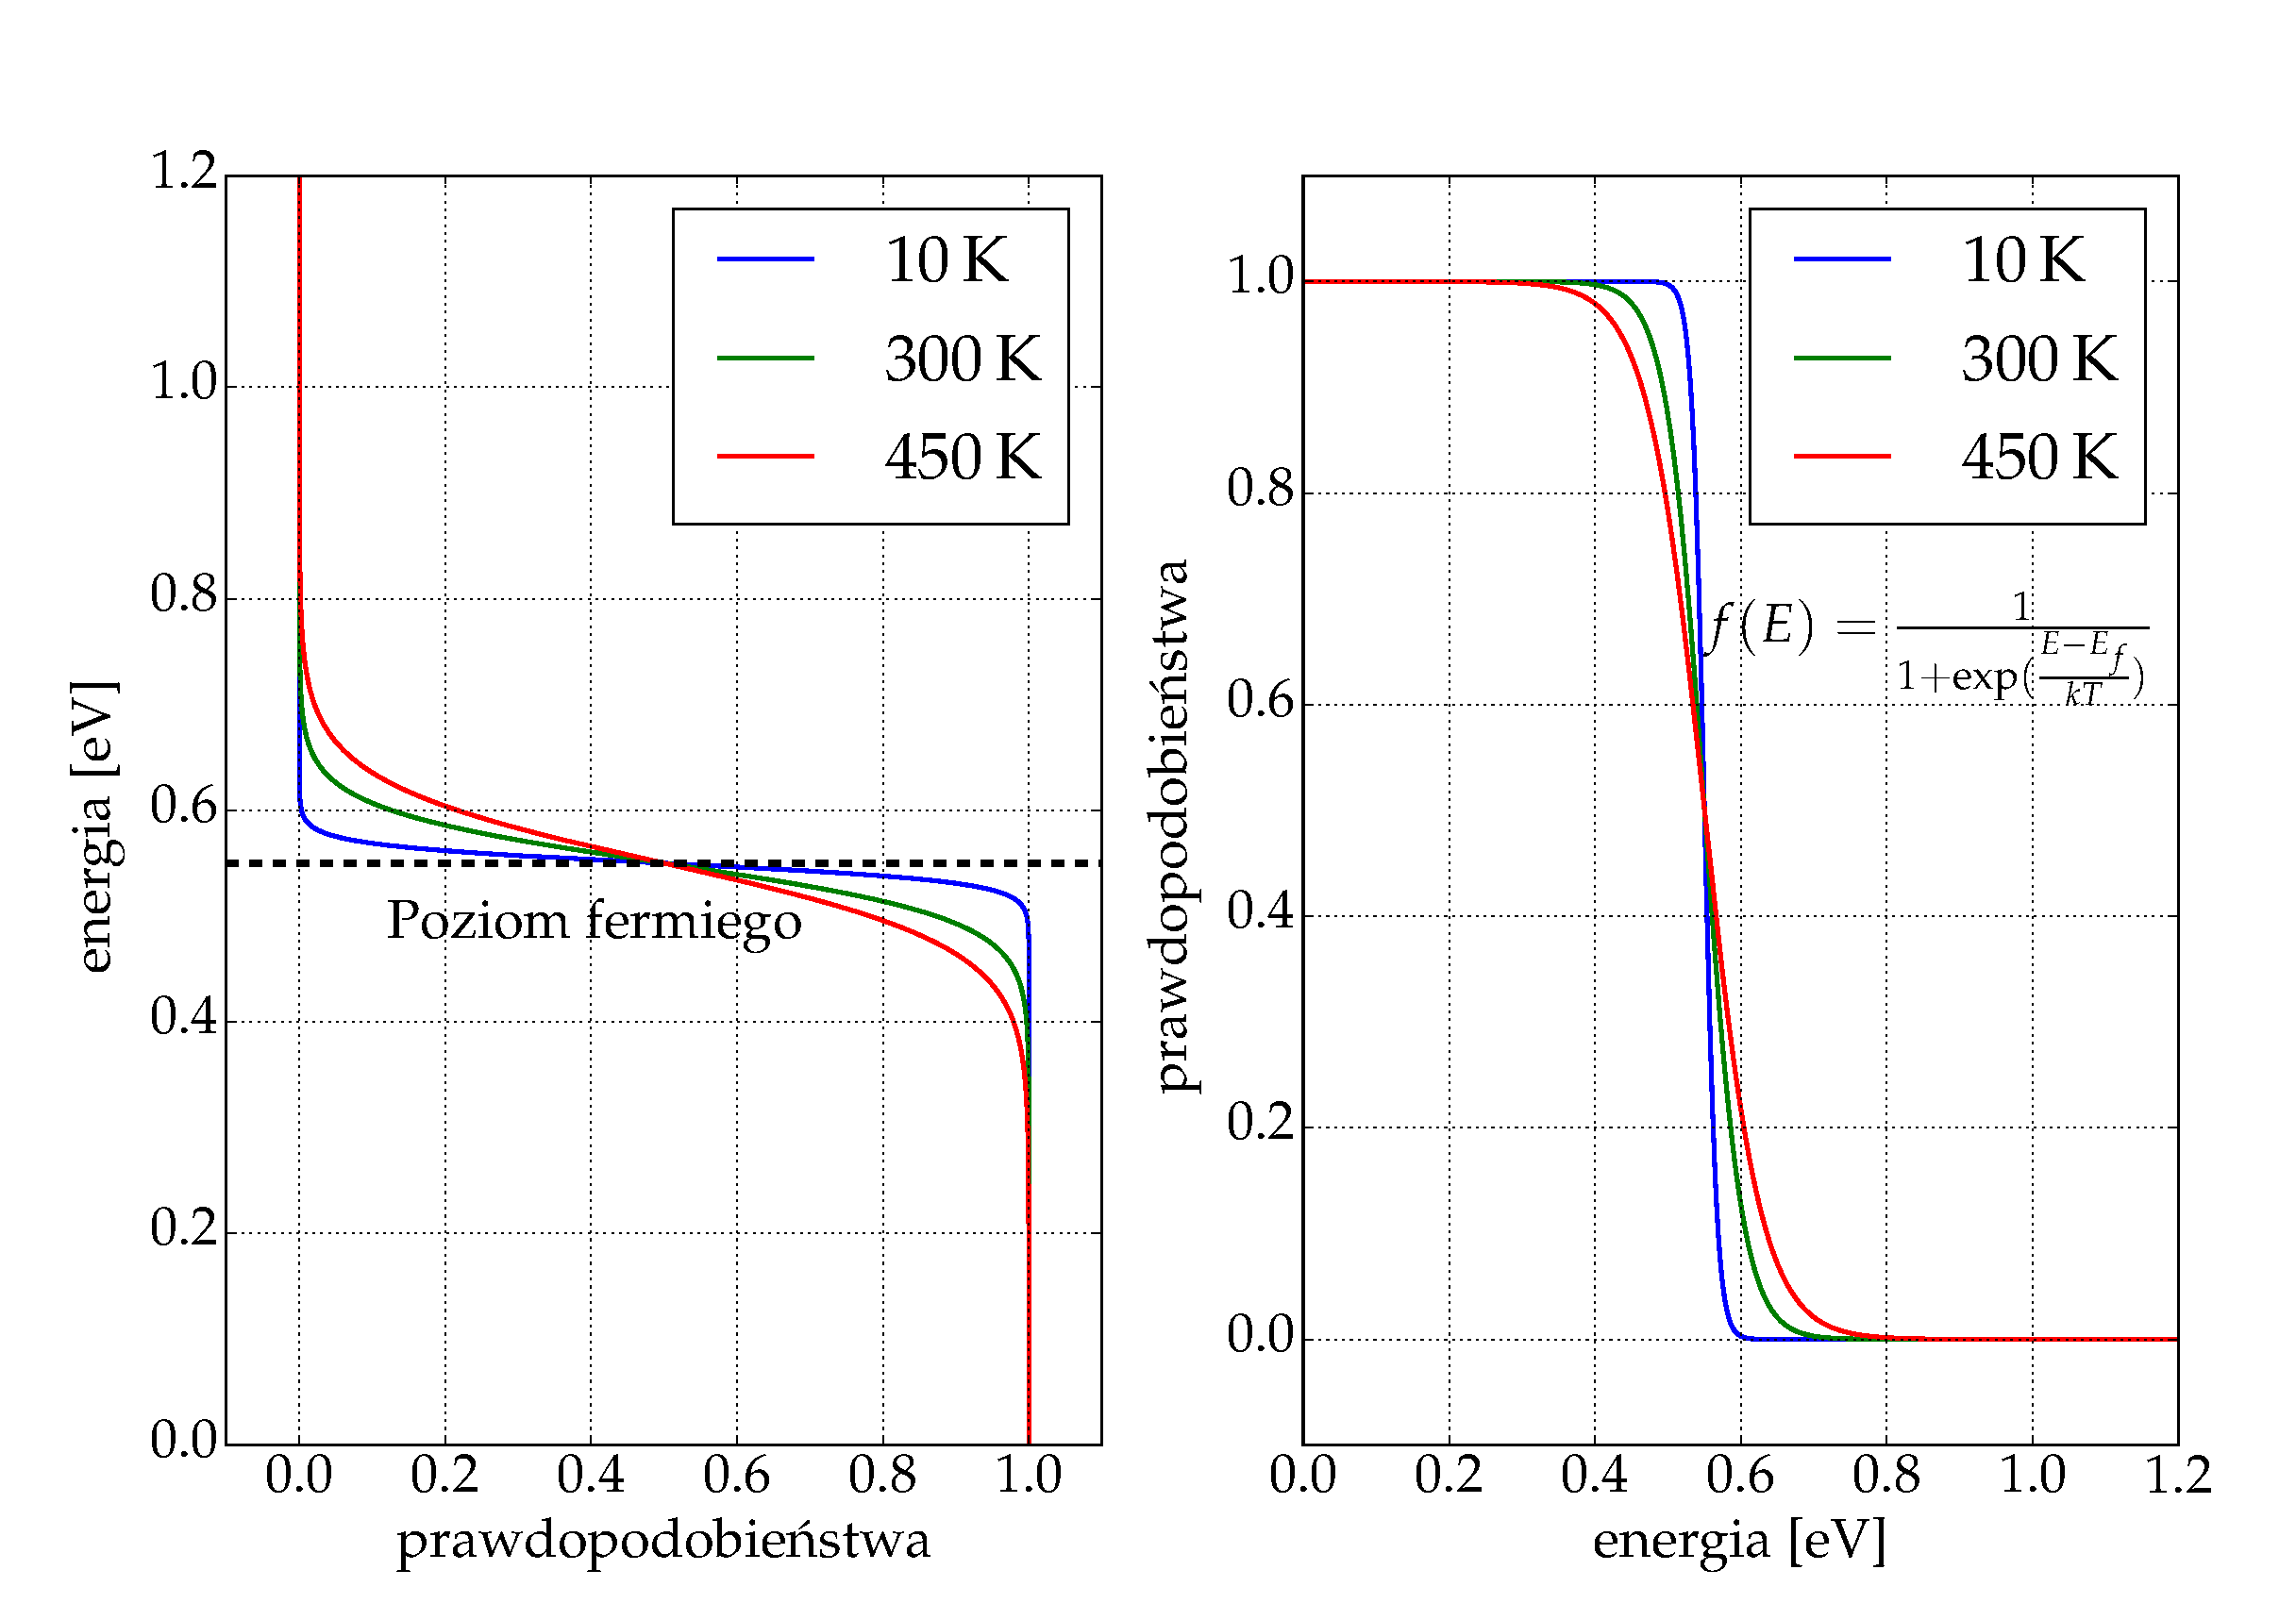
\includegraphics[scale=0.25]{fermi.eps}
  \caption{Rozkład fermiego dla różnych temperatur $T$.}
  \label{fig:teoria_rys_3}
\end{figure}
